\section{Permutation Invariance}
\begin{frame}{}
    \LARGE Advanced Computer Vision: \textbf{Permutation Invariance}
\end{frame}

\begin{frame}{Permutation Invariance}
\begin{figure}
\centering
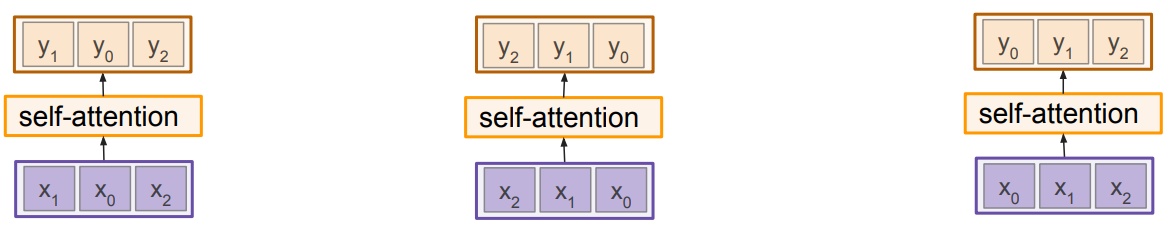
\includegraphics[width=1.0\textwidth,height=1.0\textheight,keepaspectratio]{images/advanced-cv/attention_31.png}
\end{figure}

\begin{itemize}
    \item Self-Attention Layer is Permutation equivariant
    \item It doesn’t care about the orders of the inputs!
    \item \textbf{Problem:} How can we encode ordered sequences like language or spatially ordered image features?
\end{itemize}
    
\end{frame}

\begin{frame}{Positional encoding}
\begin{itemize}
    \item Concatenate/add special positional encoding $p_j$ to each input vector $x_j$
    \item We use a function pos: $N \rightarrow \mathbb{R}^D$ to process the position $j$ of the vector into a d-dimensional vector
    \item So, $p_j = pos(j)$

\end{itemize}
\begin{figure}
\centering
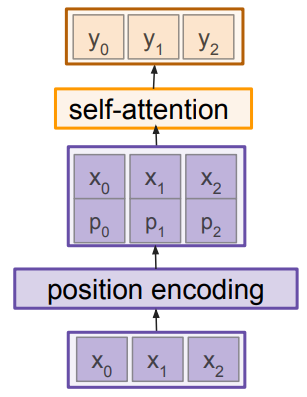
\includegraphics[width=1.0\textwidth,height=0.6\textheight,keepaspectratio]{images/advanced-cv/attention_32.png}
\end{figure}

    
\end{frame}

\begin{frame}{Masked self-attention layer}
\begin{columns}
    
    \begin{column}{0.6\textwidth}
    \only<1>{
    \begin{figure}
    \centering
    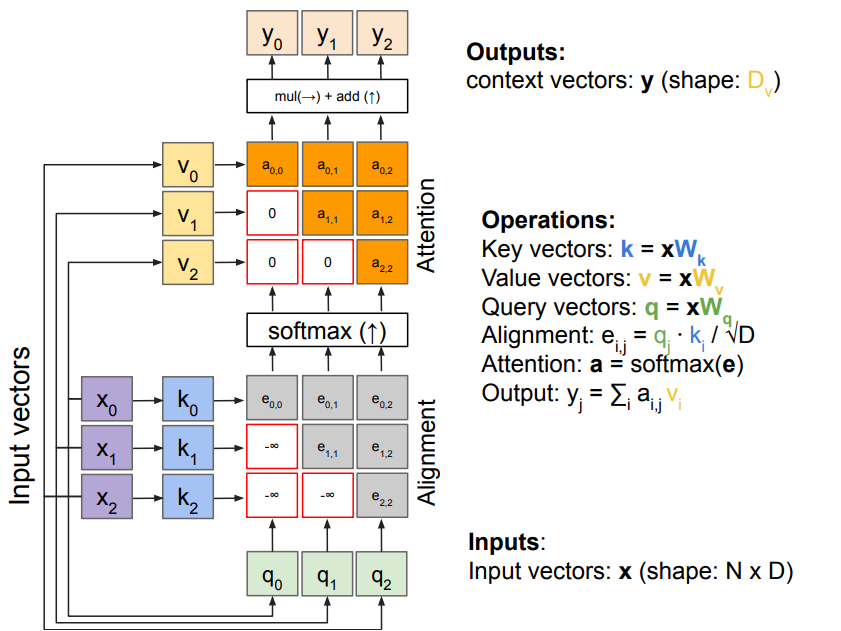
\includegraphics[width=1.0\textwidth,height=1.0\textheight,keepaspectratio]{images/advanced-cv/attention_33.png}
    \end{figure}
    }
        
    \end{column}

    \begin{column}{0.5\textwidth}
    \only<1>{
    \begin{itemize}
        \item Prevent vectors from looking at future vectors.
        \item Manually set alignment scores to $-\infty$
    \end{itemize}
    }
    
    \end{column}
\end{columns}
\end{frame}

\begin{frame}{Multi-head self-attention layer}
\begin{itemize}
    \item Multiple self-attention heads in parallel

\end{itemize}
\begin{figure}
\centering
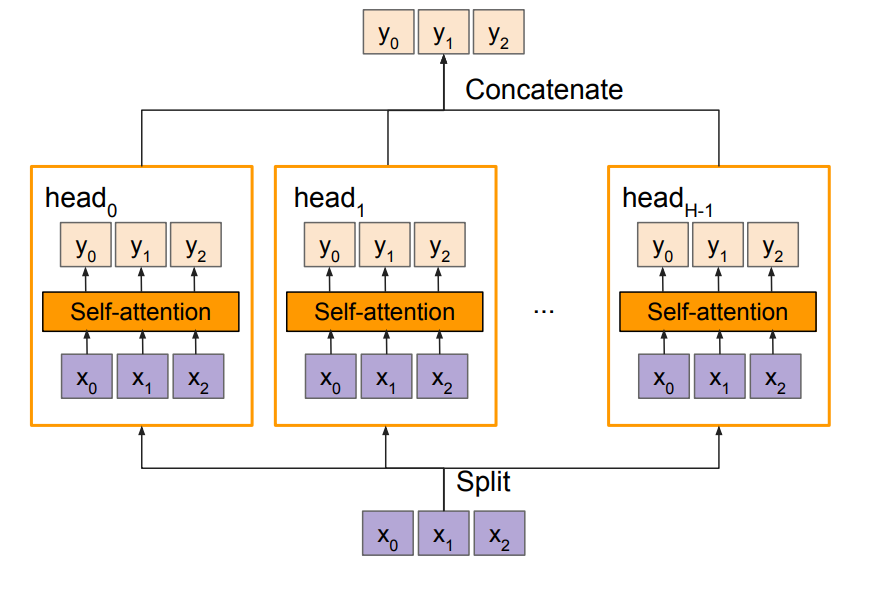
\includegraphics[width=1.0\textwidth,height=0.8\textheight,keepaspectratio]{images/advanced-cv/attention_34.png}
\end{figure}
\end{frame}

\begin{frame}{General attention versus self-attention}
\begin{figure}
\centering
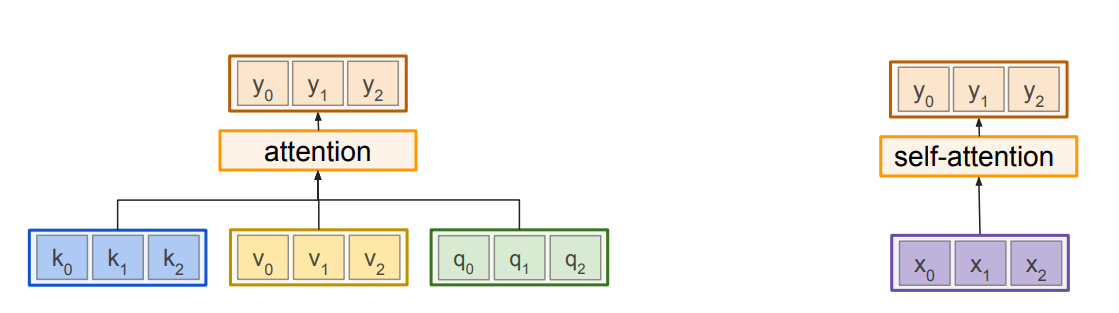
\includegraphics[width=1.0\textwidth,height=0.8\textheight,keepaspectratio]{images/advanced-cv/attention_35.png}
\end{figure}
    
\end{frame}

\begin{frame}{Example: CNN with Self-Attention}
\only<1>{
\begin{figure}
\centering
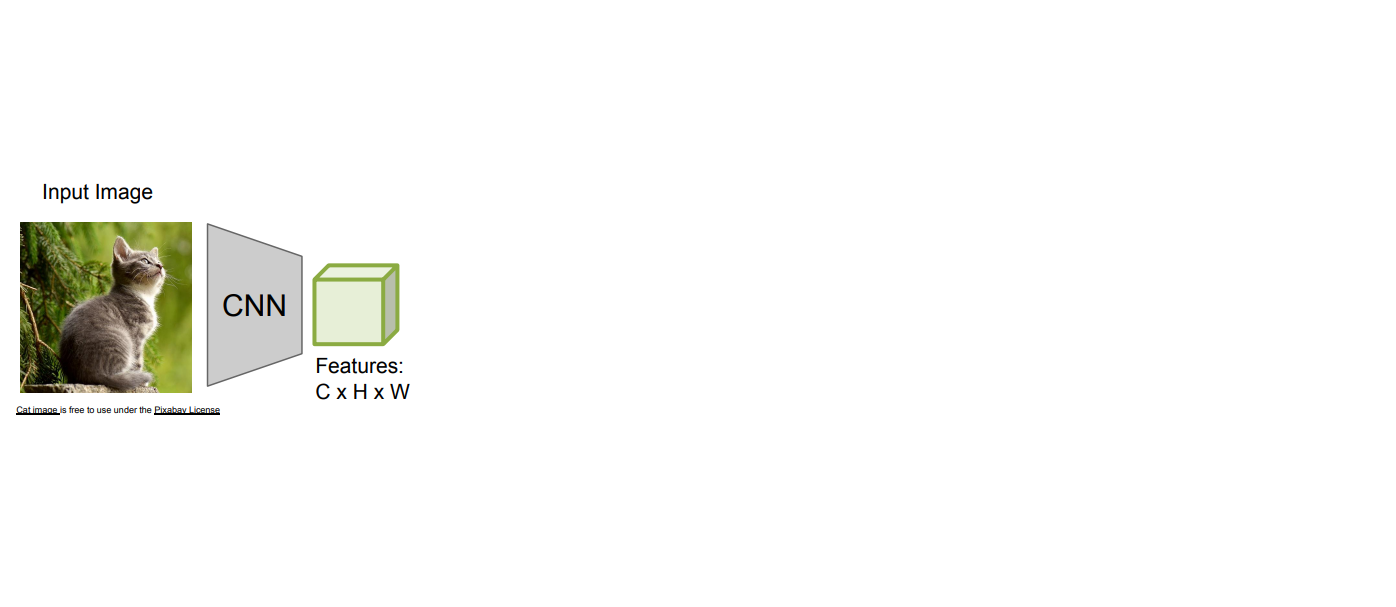
\includegraphics[width=1.0\textwidth,height=1.0\textheight,keepaspectratio]{images/advanced-cv/attention_36.png}
\end{figure}  
}

\only<2>{
\begin{figure}
\centering
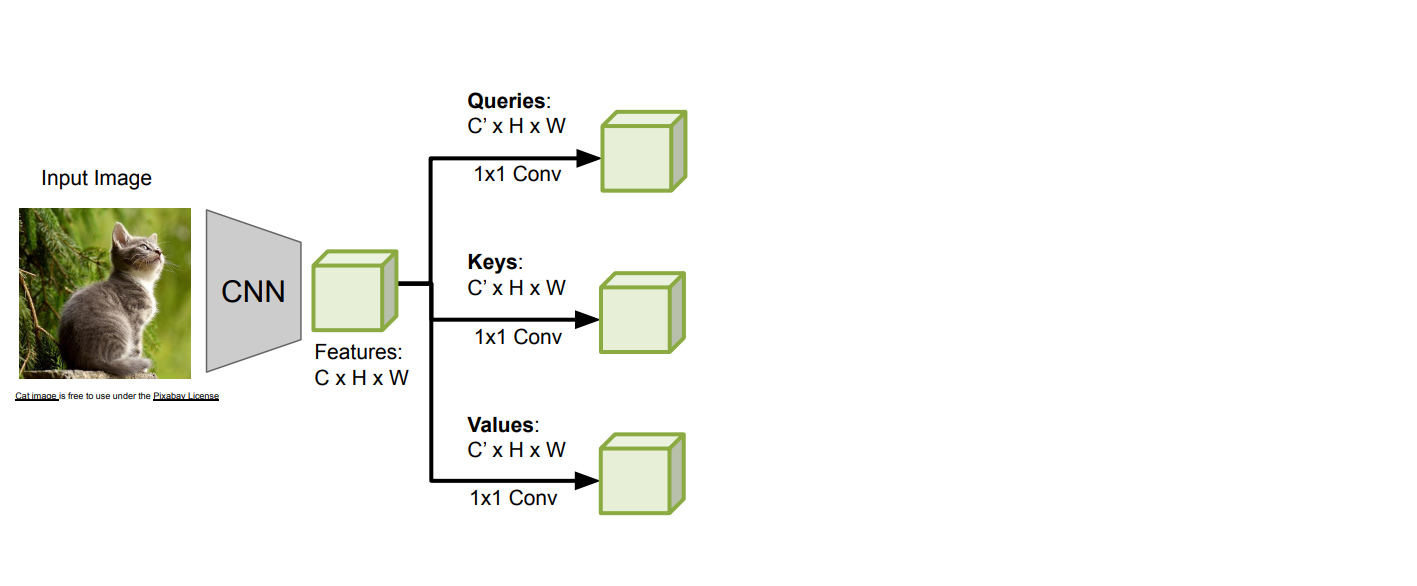
\includegraphics[width=1.0\textwidth,height=1.0\textheight,keepaspectratio]{images/advanced-cv/attention_37.png}
\end{figure}  
}

\only<3>{
\begin{figure}
\centering
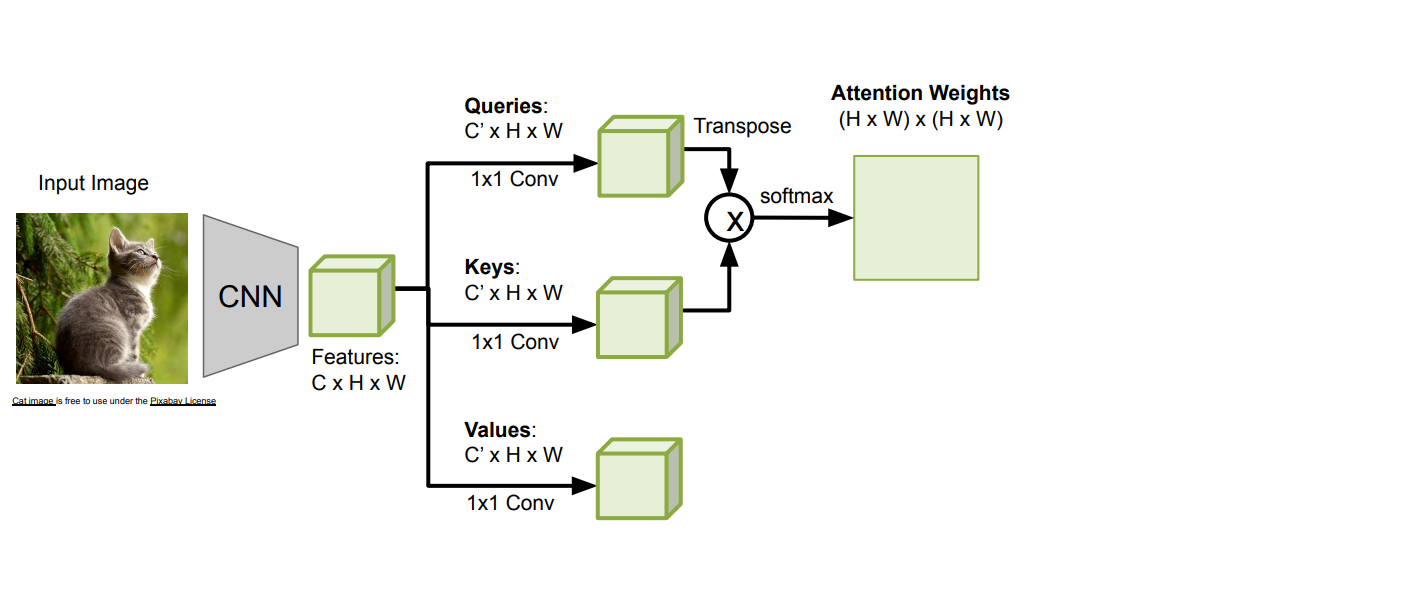
\includegraphics[width=1.0\textwidth,height=1.0\textheight,keepaspectratio]{images/advanced-cv/attention_38.png}
\end{figure}  
}

\only<4>{
\begin{figure}
\centering
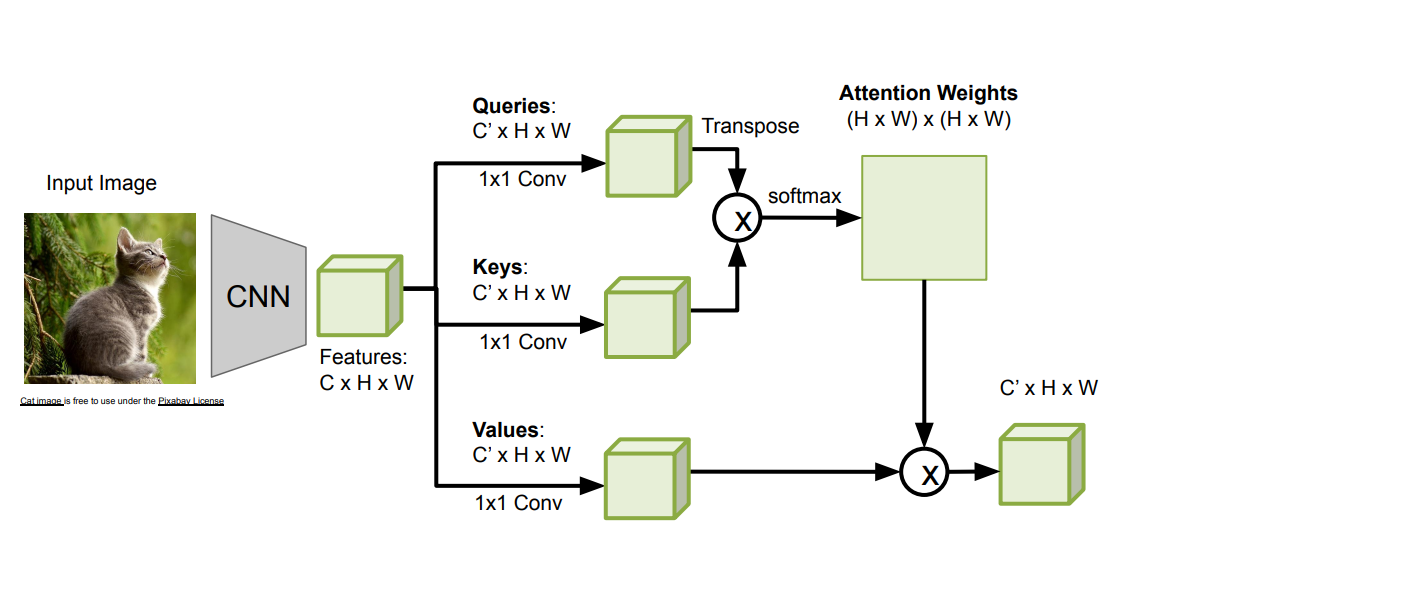
\includegraphics[width=1.0\textwidth,height=1.0\textheight,keepaspectratio]{images/advanced-cv/attention_39.png}
\end{figure}  
}

\only<5>{
\begin{figure}
\centering
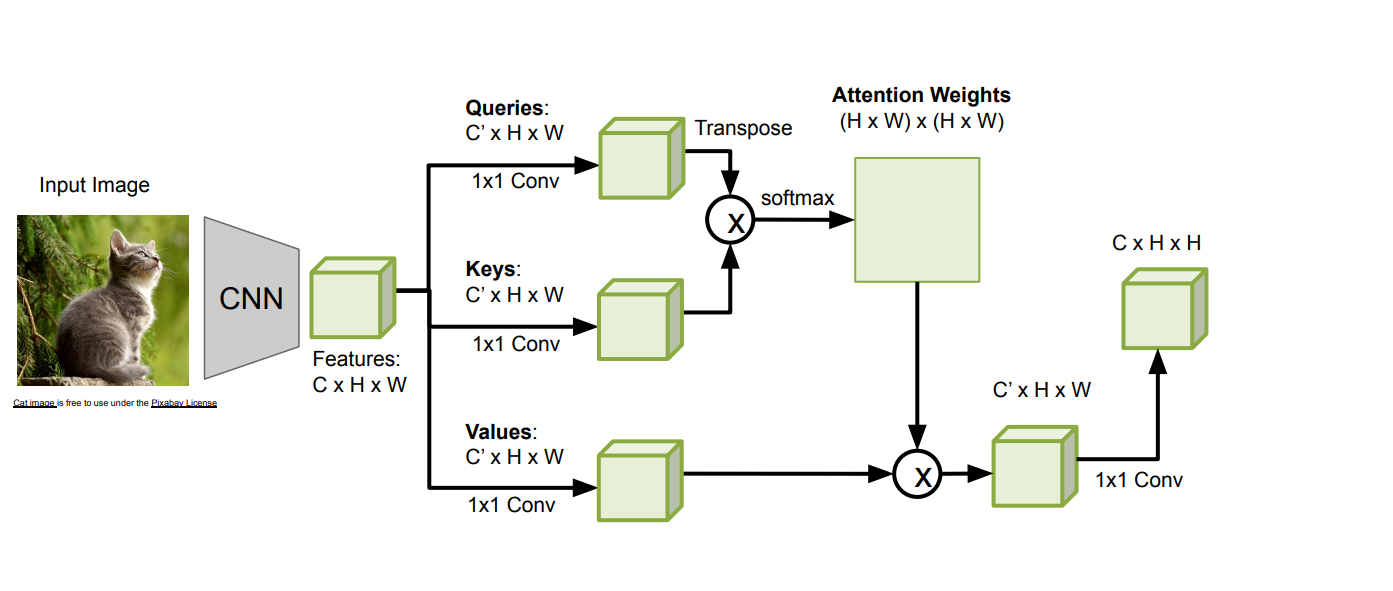
\includegraphics[width=1.0\textwidth,height=1.0\textheight,keepaspectratio]{images/advanced-cv/attention_40.png}
\end{figure}  
}

\only<6>{
\begin{figure}
\centering
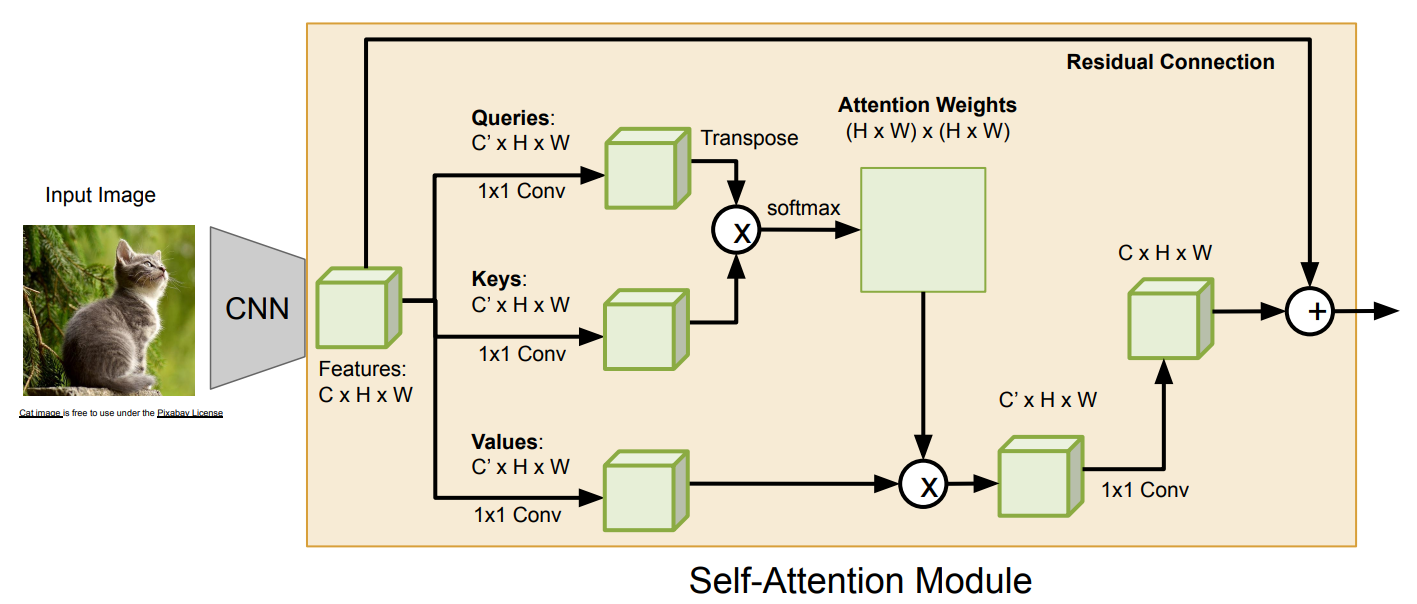
\includegraphics[width=1.0\textwidth,height=1.0\textheight,keepaspectratio]{images/advanced-cv/attention_41.png}
\end{figure}  
}
\end{frame}